\documentclass[dvipsnames]{beamer}
\input{mybeamerdefs}
\title{MRI Simulator Notes}
\author{Liam}
\date{\today}

\begin{document}

\begin{frame}
\maketitle
\end{frame}

\begin{frame}{Tasks}
\begin{itemize}
\item I debugged my 2DFT simulation + reconstruction and ran it with a few different em distributions.
\end{itemize}
\end{frame}

\section{2DFT simulation + reconstruction}

\begin{frame}{Summary}
\begin{itemize}
\item I distributed ems in the plane $z = 0$, ran the simulation with a 2DFT pulse sequence, and reconstructed the image.
\item The em distributions and corresponding reconstructions are shown in the figures below.
\end{itemize}
\end{frame}

\begin{frame}
\begin{center}
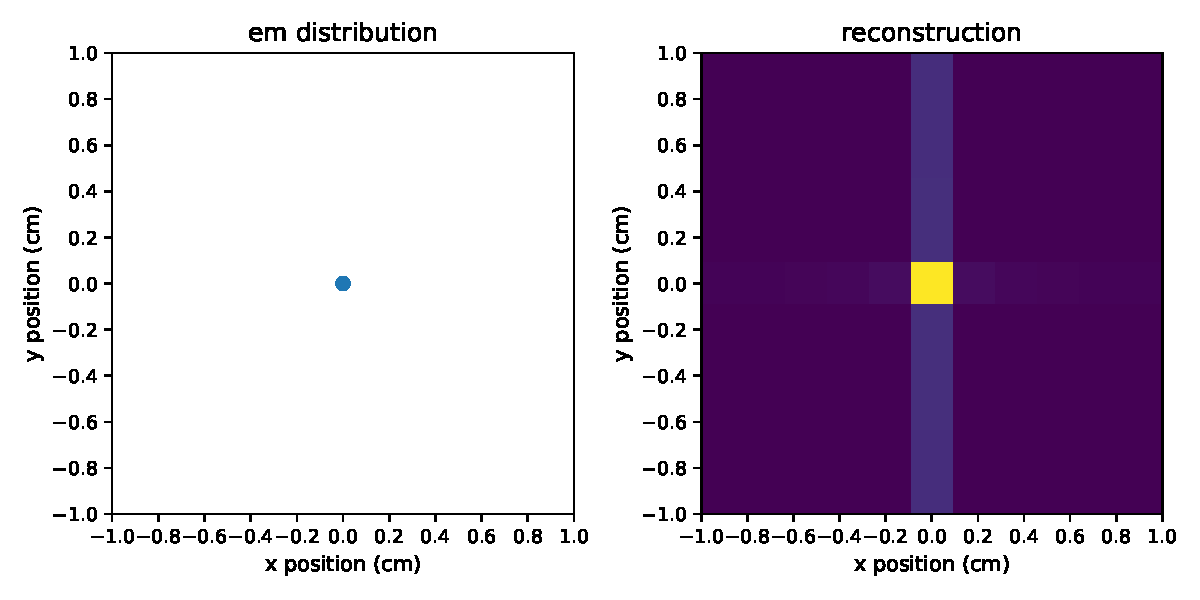
\includegraphics[width=\textwidth]{reconstruction_ems-origin}
\end{center}
\end{frame}

\begin{frame}
\begin{center}
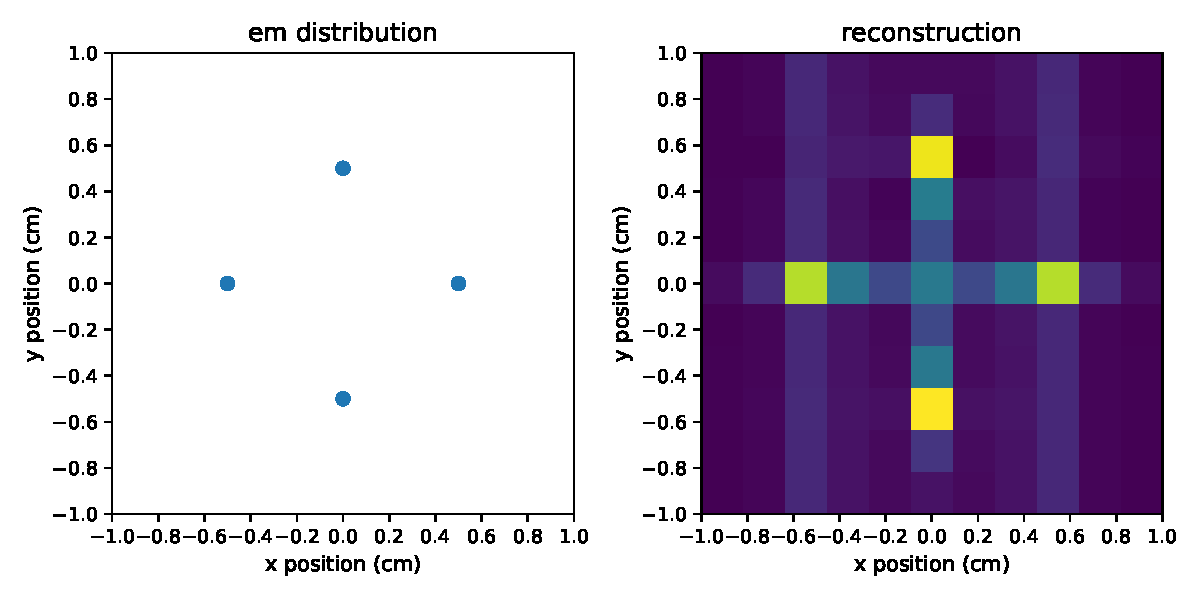
\includegraphics[width=\textwidth]{reconstruction_ems-star}
\end{center}
\end{frame}

\begin{frame}
\begin{center}
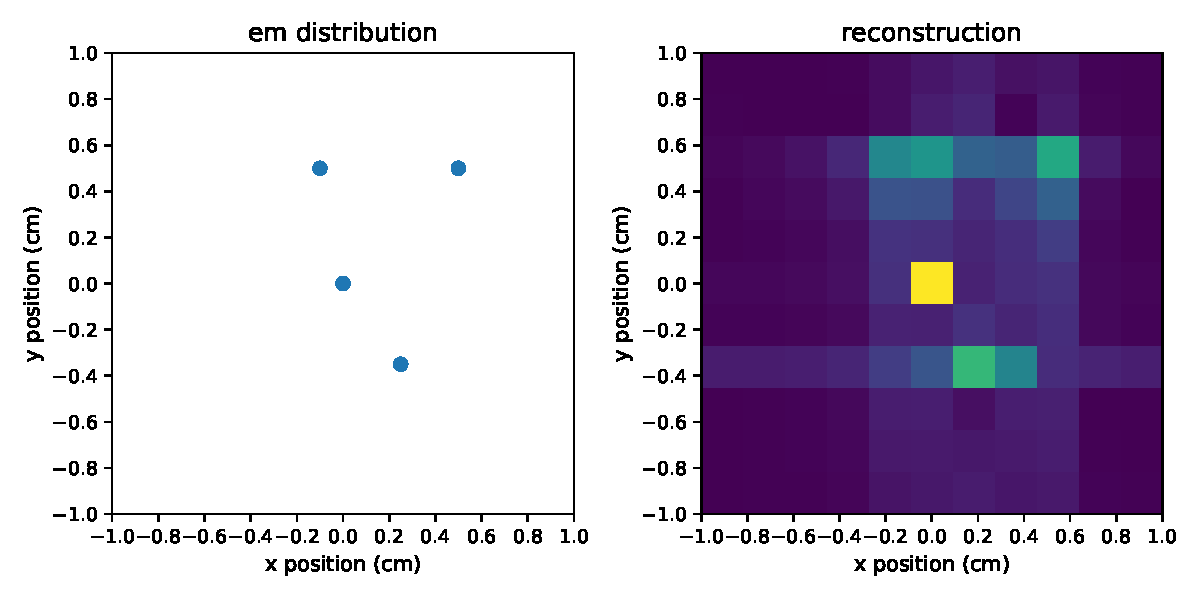
\includegraphics[width=\textwidth]{reconstruction_ems-scattered}
\end{center}
\end{frame}

\begin{frame}{Comments}
\begin{itemize}
\item The images are consistent with the em distributions.
\item I'm not sure why there is asymmetric blurring of the images.
\item Could it have to do with relaxation? I am incorporating relaxation with T1 = 10 ms, T2 = 10 ms, TR $\approx$ 50 ms.
\end{itemize}
\end{frame}


\end{document}